\documentclass[12pt, french]{article}
\usepackage{graphicx}
\usepackage[T1]{fontenc}
\usepackage[utf8]{inputenc}
\usepackage{lmodern}
\usepackage[a4paper]{geometry}
\usepackage{babel}
\usepackage{wrapfig}
\usepackage[figurename=Fig.]{caption}
\usepackage{subfig}
\begin{document}
	\begin{titlepage}
		
		\newcommand{\HRule}{\rule{\linewidth}{0.4mm}} % Defines a new command for the horizontal lines, change thickness here
		
		\center % Center everything on the page
		
		%----------------------------------------------------------------------------------------
		%	HEADING SECTIONS
		%----------------------------------------------------------------------------------------
		
		\textsc{\LARGE Université de Montréal}\\[1cm] % Name of your university/college
		\textsc{\Large Faculté des arts et des sciences}\\[0.5cm] % Major heading such as course name
		\textsc{\large Département d’informatique et de recherche opérationnelle (DIRO) }\\[0.3cm] % Minor heading such as course title
		
		%----------------------------------------------------------------------------------------
		%	TITLE SECTION
		%----------------------------------------------------------------------------------------
		
		\HRule \\[0.4cm]
		{ \huge Rapport de stage \\ \bfseries Évaluation du risque de retour à la maison } \\[0.4cm] % Title of your document
		\HRule \\[1.5cm]
		
		%----------------------------------------------------------------------------------------
		%	AUTHOR SECTION
		%----------------------------------------------------------------------------------------
		
		\begin{minipage}{0.4\textwidth}
			\begin{flushleft} \large
				\emph{Auteur:}\\
				Vilon \textsc{Saint-Fleurose} % Your name
				\\MSc, informatique \\Université de Montréal
			\end{flushleft}
		\end{minipage}
		~
		\begin{minipage}{0.4\textwidth}
			\begin{flushright} \large
				\emph{Directeur de recherche:} \\
				Dr. Michalis \textsc{Famelis} % Supervisor's Name
				\\Professeur adjoint \\Université de Montréal
			\end{flushright}
		\end{minipage}\\[1cm]
			~
			\begin{minipage}{0.4\textwidth}
				\begin{center} \large
					\emph{Superviseur:} \\
					 Nicolas \textsc{Coallier} % Supervisor's Name
					\\Vice-Président Exécutif, TIC \\ML+
				\end{center}
			\end{minipage}\\[1cm]
		
		% If you don't want a supervisor, uncomment the two lines below and remove the section above
		%\Large \emph{Author:}\\
		%John \textsc{Smith}\\[3cm] % Your name
		
		%----------------------------------------------------------------------------------------
		%	DATE SECTION
		%----------------------------------------------------------------------------------------
		
		{\large \today}\\[1cm] % Date, change the \today to a set date if you want to be precise
		
		%----------------------------------------------------------------------------------------
		%	LOGO SECTION
		%----------------------------------------------------------------------------------------
		
		
\includegraphics[width=3cm, height=1cm]{logo.png} % Include a department/university logo - this will require the graphicx package
		
		%----------------------------------------------------------------------------------------
		
		\vfill % Fill the rest of the page with whitespace
		
	\end{titlepage}
	
	\section*{Remerciements}
	Je veux commencer d'abord par remercier le Grand Dieu Tout-Puissant, le Créateur de l'univers, des cieux et de la terre qui m'a donné la vie, la santé, les opportunités et tout ce dont j'avais besoin pour faire cette grande et belle étude à l'université de Montréal. Il a rendu toutes choses possibles en ma faveur, moi qui suis pécheur et désobéissant; immérité de toutes ces grâces. Il m'accompagnait toujours dans les moments les plus difficiles de ma vie, Il ne m'a jamais laissé seul; surtout dans les moments où je devais payer les frais de scolarité qui étaient si énormes et impossibles à payer de mon propre compte. A un Dieu si merveilleux et si bon, je Lui dois beaucoup de reconnaissance.  \\
	
	Je remercie aussi ma femme qui m'a beaucoup supporté pendant plus de deux années d'études. Elle n'a jamais murmuré, ni découragé quand nous devions passer par des moments difficiles de notre vie conjugale à cause de ces études. Elle a mis toutes ses ressources disponibles pour entretenir la famille et payer mes études quand j’étais moi-même dans l’impossibilité de travailler. Vraiment, ma femme est une bénédiction dans ma vie, un cadeau venant de Dieu. Je t’aime ma chérie. \\
	
	Je tiens à remercier le professeur Michalis Famelis d’avoir accepté être mon directeur de recherche et supervisé ce stage, il est toujours là pour m’encourager et me pousser vers l’avant. Il répond toujours présent à tous mes appels, il est toujours disponible pour me rencontrer, me parler et me conseiller ; même en dehors du cadre universitaire.  \\
	
	Je remercie Nicolas Coallier et toute l’équipe ML+ qui ont accepté que je sois leur stagiaire, ils ont placé  leur confiance en moi quoiqu’ils ne me connaissaient pas encore. Cette équipe, quoique jeune, est très dynamique et chaleureuse, c’est une équipe motivante qui stimule la connaissance. J’ai dû apprendre beaucoup de choses par rapport à eux.
	Finalement, je présente mes sincères remerciements à toute la communauté universitaire, à DIRO en particulier. Merci pour la formation prestigieuse que vous m’avez fournie. Cette formation est si solide qu’elle m’aidera rapidement à intégrer le marché du travail sans perdre de temps. 
	
\newpage
	
\section*{Résumé}
L'arthroplastie totale de la hanche et du genou réduit considérablement la douleur
et améliore la fonction chez les personnes atteintes d'arthrose avancée. le
vieillissement de la génération du "baby boom", combiné au désir de
maintenir un mode de vie actif et sans douleur, entraînera une augmentation
le nombre annuel de chirurgies de remplacement articulaire pratiquées dans
États Unis. L'Académie américaine des chirurgiens orthopédiques a
projeté que d'ici 2030, les arthroplasties totales de la hanche et du genou
augmentera à plus de 748 000 / an. 
Avec l'augmentation continue du nombre de chirurgies de remplacement, il devient essentiel aux administrateurs des hôpitaux de déterminer si les patients doivent rester à l'hôpital pour une réadaptation après leur 	chirurgie ou s'ils doivent être renvoyés à la maison. Il est important de souligner que la majorité des compagnies d'assurance santé aux États Unis n'assument pas les coûts liés à la réhabilitation des patients. Ces frais qui sont très élevés (entre 15-30,000 \$ par patient) doivent être assurés par les hôpitaux. Pour prendre la décision de retour ou non, les chirurgiens tiennent compte des antécédents médicaux du patient. Dans notre projet de stage, nous développerons un model de maching learning qui aide à prendre cette décision de façon automatique.
   	
\newpage
\section{Introduction}	
	
Le système de santé aux USA repose sur deux types de financement. Premièrement, sur le financement public qui englobe certains groupes de personnes de la population américaine uniquement. Il se concentre 	essentiellement sur deux programmes : le programme 		fédéral Medicare pour les plus de 65 ans et les personnes gravement handicapées (soit 15 \% de la population) et le programme Medicaid qui 			s’adresse aux familles pauvres avec enfants et touche 11 \% de la population. Deuxièmement, sur le financement privé qui touche tout le reste de la population, l’assurance est donc majoritairement privée aux 		Etats-Unis. Les Américains sont assurés en général via leurs employeurs ou sinon de manière individuelle lorsque leur employeur ne propose pas d’assurance ou qu’ils travaillent en indépendant. La composante « 	assurance médicale » dans le choix d’un emploi est donc un critère important.\\
	
Le système américain, libéral et fondé sur le marché, s’organise autour d’assurances privées souvent liées à l’emploi et d’une assurance maladie obligatoire, liée notamment à la vieillesse et aux faibles revenus.
Cependant, ce système, qui n’est pas universel, échoue à couvrir l’intégralité de la population, dont une partie se retrouve sans assurance santé.\\

Les compagnies d'assurance privées ne couvrent pas les coûts associés à une réadaptation d'un patient après une arthroplastie (Opération ayant pour but de rétablir la forme et la mobilité d'une articulation abîmée ou bloquée.). Il revient à l'hôpital de couvrir ces coûts qui sont très élevés d'après le docteur orthopédiste Jonah Hebert-Davies qui a fait ses études de spécialité en Orthopédie à l'université de Seattle, Washington USA. Selon le docteur les coûts estimés sont entre 15 à 30,000 \$ par patient. Ce qui revient à une grande perte financière pour les hôpitaux.  La décision de maintenir ou de renvoyer un patient après une arthroplastie devient une question préoccupante dans la mesure où elle pourrait réduire le coût budgétaire des hôpitaux. Si la décision prise est de renvoyer le patient, l'hôpital est le gagnant sinon il est le perdant\\ 

D'autres part, l'arthrose (maladie qui touche les articulations et caractérisée par la douleur et la difficulté à effectuer des mouvements articulaires) touche environ 27 millions d'adultes aux États-Unis.  Ce qui augmente considérablement le nombre d'arthroplastie dans les hôpitaux, et aussi le poids de travail des médecins à savoir quand est-ce qu'il ya une réadaptation ou non.\\

Il est un travail fastidieux pour les spécialistes orthopédistes de vérifier manuellement les données médicales d'un patient pour pouvoir décider s'il doit être renvoyé ou non. Ce travail consiste en ce que les données médicales d'un dossier patient sont très volumineuses. Créer un moyen d'automatiser ce processus est le but de notre projet.  \\

Nous supposons qu'il existe déjà un jeu de données disponibles contenant toutes les informations touchant un grand nombre de patients et que chaque échantillon de ce jeu de données est un dossier patient. Nous supposons aussi que ce jeu de données possède des caractéristiques suffisantes pour décider si un patient doit être renvoyé ou non. Nous considérons aussi que ce jeu de données est composé de patients qui font l'objet d'une décision de retour. Si toutes ces conditions sont réunies, nous pouvons profiter des technologies de la science de données en général et du marching learning en particulier pour créer un outil d'aide à la décision qui aide les orthopédistes à prendre la décision de retour automatiquement. \\

La suite de ce rapport est composé de plusieurs sections et chaque section peut avoir des subsections. La section 2 donne un contexte théorique des différents éléments qui sont importants pour notre projet. La section 3 présente en détail une description technique des différentes étapes de notre projet. La section 4 fait une évaluation de notre outil crée. La section 5 présente les limitations et les travaux futurs. La section 6 détaille les travaux connexes et la section 7 est celle de la conclusion.


\newpage

\section{Contexte théorique}

Dans cette section nous voulons présenter une approche théorique des différents concepts que nous avons utilisés dans le cadre notre projet. Nous allons faire un résumé de chaque concept important que nous avons utilisé dans le cadre de l'implémentation de ce projet. Nous n'allons pas toucher tout ce qui a rapport aux concepts mais juste ce qui nous intéresse et util pour le projet. Il y aura des références pour ceux qui veulent approfondir les concepts. 

\subsection{Sciences des données}

La science des données est un domaine interdisciplinaire de méthodes, processus, algorithmes et systèmes scientifiques permettant d'extraire des connaissances ou des informations à partir de données sous diverses formes, structurées ou non. Elle emploie des techniques et des théories tirées de plusieurs autres domaines plus larges des mathématiques, la statistique principalement, la théorie de l'information et la technologie de l'information, notamment le traitement de signal, des modèles probabilistes, l'apprentissage automatique, l'apprentissage statistique, la programmation informatique, l'ingénierie de données, la reconnaissance de formes et l'apprentissage, la visualisation, l'analytique prophétique, la modélisation d'incertitude, le stockage de données, la compression de données et le calcul à haute performance. Les méthodes qui s'adaptent aux données de masse sont particulièrement intéressantes dans la science des données, bien que la discipline ne soit généralement pas considérée comme limitée à ces données.\\
	
L'objectif du « data scientist » (expert en données massives) est de produire des méthodes (automatisées, autant que possible) de tri et d'analyse de données de masse et de sources plus ou moins complexes ou disjointes de données, afin d'en extraire des informations utiles ou potentiellement utiles. 
Le métier de data scientist est apparu pour trois raisons principales :	
\begin{itemize}
\item l'explosion de la quantité de données produites et collectées par les humains;
\item 	l'amélioration et l'accessibilité plus grande des algorithmes de machine learning;
\item l'augmentation exponentielle des capacités de calcul des ordinateurs.\\
\end{itemize}	
Le cycle de travail du data scientist comprend notamment:
\begin{itemize}
\item la récupération des données utiles à l'étude;
\item le nettoyage des données pour les rendre exploitables;
\item une longue phase d'exploration des données afin de comprendre en profondeur l'articulation des données;
\item la modélisation des données;
\item l'évaluation et interprétation des résultats;
\item  la conclusion de l'étude : prise de décision ou déploiement en production du modèle.
\end{itemize}
L'image ci-dessous donne une vue du travail du data scientist. Étant stagiaire en science de données, nous avons suivi minitieusement, dans le cadre de notre projet, le cycle de travail complet du data scientist. Depuis la récupération des données jusqu'au déploiement d'un système en production. Nous expliquerons en détail dans la section "Aperçu", comment nous implémentons ce cycle au sein de notre projet. \\ \\

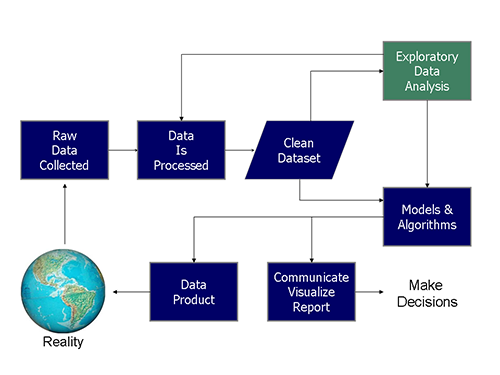
\includegraphics{workflow_datascientis.png}


Deux composantes sont nécessaires pour pouvoir commencer à se demander si la data science peut, oui ou non, apporter de la valeur et aider à la résolution d'un problème : des \textbf{données} et une \textbf{problématique} bien définie.\\\\ 
Les données constituent la ressource principale pour qu'un data scientist puisse effectuer son travail correctement. Nos données proviennent du département orthopédique de l'université de Seattle, Washington, États-Unis. Elles sont au nombre de 2718 files et 92 colonnes. Nous les utilisons comme données historiques (\textit{historical data, en anglais}) dans le cadre du développement de notre modèle de machine learning. \\ 
La problématique de notre projet, comme nous l'avons vu dans l'introduction, est d'aider à décider si un patient doit rester à l'hôpital ou rentrer chez lui après une arthroplastie.  

Au sein de ce cycle, le machine learning désigne l'ensemble des méthodes de modélisation statistique à partir des données, et se situe bien au coeur du travail de data scientist.\\

\subsection{Machine Learning}

Dans la section précédente, nous avons pu y voir plus clair sur le cycle global de travail du data scientist. Nous allons maintenant parler du machine learning dans cette section, c'est à dire la modélisation des données. Le machine learning constitue une manière de modéliser des phénomènes, dans le but de prendre des décisions stratégiques.




\newpage

\section{Aperçu}
\subsection{Obtention des données}
\subsection{Nettoyage des données}
\subsection{Exploration des données}
\subsection{Modélisation des données}


\newpage

\section{Évaluation}


\newpage

\section{Limitations et travaux futurs}

\newpage

\section{Travaux connexes}


\newpage

\section{Conclusion}
	
\end{document}
